% Number 260
% CVPMA Algebra Units
% Model discrimination, avg v/speed
% JG

% Watermark
\AddToShipoutPicture*{\BackgroundPic}

\addtocounter {ProbNum} {1}

%\begin{floatingfigure}[r]{.3\textwidth}
%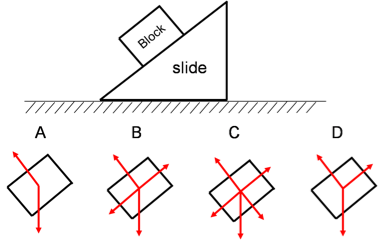
\includegraphics[scale=.4]{/Users/jgates/desktop/latex/pics/incline3.png}
%\end{floatingfigure}
 
{\bf \Large{\arabic{ProbNum}}} A ball is thrown vertically into the air.  It takes 2.42 seconds for it to reach its peak height of 24.5 meters.

\bigskip
Does CVPM apply? Why or why not?

\vspace{30mm}
What was the ball's average velocity during the trip to the peak of its motion?

\vfill
The ball will take another 2.42 seconds to hit the ground.  What is its average velocity over the whole trip?

\vfill
What was the ball's average speed during the whole trip?

%\begin{center}
%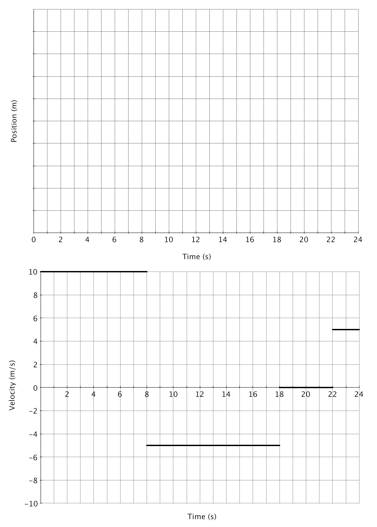
\includegraphics[scale=.77]{/Users/jgates/desktop/latex/pics/vtoxgraph1.png}
%\end{center}
 
\vfill

\newpage